\chapter{Weiterführende Informationen}\label{app:supplemental-information}

\section{Reed-Solomon mit BCH-Schema}\label{app:bch-rs}

Das Reed-Solomon-Verfahren basiert auf dem \acrfull{bch}-Schema und arbeitet wie der ursprüngliche Reed-Solomon-Code im Galois-Feld $GF(2^r)$.
Die Daten werden als Polynom $p(x)$ über diesem Galois-Körper dargestellt. 
Um das Codewort zu erzeugen, wird dieses Nachrichtenpolynom $p(x)$ mit einem Generatorpolynom $g(x)$ multipliziert \cite{stoneMultipleBurstErrorCorrection1963}.
\[
c(x)=p(x)g(x)
\]
Dieses Generatorpolynom wird bei der Spezifizierung der Ausprägung des eingesetzen Verfahrens festgelegt und ist somit beim En- und Decodieren bekannt \cite{deepak2018WhatReedSolomon2022}.

Das Codepolynom $c(x)$ wird durch dessen Koeffizienten an den Empfänger übertragen oder auf ein Medium gespeichert.
Zum Decodieren wird die Encodierungsgleichung nach $p(x)$ aufgelöst und dann wird $p(x)=\frac{c(x)}{g(x)}$ mit Hilfe von Polynomdivision bestimmt \cite{geiselTutorialReedSolomonError1990}.

\section{Beweis des Hamming-Abstands von Reed-Solomon-Codes}\label{app:hammingDistanceRS}

Wie schon in Abschnitt \ref{sec:decoding} auf Seite \pageref{sec:decoding} erwähnt, sind zum Decodieren eines Codeworts $\binom{n}{k}$ Gleichungssysteme möglich.
Davon führen $\binom{n-t}{k}$ Gleichungssysteme zur richtigen Lösung.
$\binom{t+k-1}{k}$ Gleichungssysteme, die mindestens eine fehlerbehaftete Gleichung enthalten, ergeben jeweils falsche Lösungen.
Von all diesen Lösungen wird diejenige ausgewählt, welche am häufigsten aufgetreten ist und damit korrekt ist.
Damit diese Entscheidung erfolgreich die richte Lösung auswählt, muss also $\binom{n-t}{k} > \binom{t+k-1}{k}$ sein \cite{reedPolynomialCodesCertain1960}.
Durch Umformung entsteht folgende Ungleichung, die für $n$, $k$ und $t$ erfüllt sein muss, damit das Reed-Solomon-Verfahren funktioniert.
\begin{align}
\binom{n-t}{k} &> \binom{t+k-1}{k} \nonumber\\
n-k+1 &> 2t \nonumber
\end{align}
Das bedeutet, dass es nie $n-k+1$ oder mehr Fehler geben darf \cite{reedPolynomialCodesCertain1960}.
Das entspricht dem Hamming-Abstand, der genau diese Obergrenze für \acrshort{ecc}s angibt.

\section{Vergleich mit anderen Codierungsverfahren}\label{app:comparison}

\begin{table}[h]
	\begin{tabular}{@{}l|cccc@{}}
		\toprule
		& \textbf{Codelänge} & \textbf{Nachrichtenlänge} & \textbf{Fehlererkennung} & \textbf{Fehlerkorrektur} \\
		& \textbf{n}         & \textbf{k}                & \textbf{2t}              & \textbf{t}               \\ \midrule
		Hamming      & 6   & 3   & 2  & 1  \\
		Reed-Solomon & 5   & 3   & 2  & 1  \\
		BCH          & 7   & 3   & 2  & 1  \\ \midrule
		Hamming      & 255 & 247 & 2  & 14 \\
		Reed-Solomon & 255 & 223 & 32 & 16 \\
		BCH          & 255 & 179 & 20 & 10 \\ \bottomrule
	\end{tabular}
	\caption{Tabelle zum Vergleich verschiedener Codierungsverfahren}
	\label{tab:comparison}
\end{table}

In Tabelle \ref{tab:comparison} werden drei gängige Codierungsverfahren - Hamming, Reed-Solomon und BCH - hinsichtlich ihrer Parameter Codelänge $n$, Nachrichtenlänge $k$, Fehlererkennung $2t$ und Fehlerkorrektur $t$ verglichen. 

Der erste Teil der Tabelle zeigt die Parameter beispielhaft für Nachrichten der Länge $k=3$. 
Dazu wurde die Codelänge so gewählt, dass alle drei Verfahren die gleiche Anzahl an Fehlern korrigieren \bzw erkennen können.
Dieses Beispiel ist nicht repräsentativ, da typischerweise längere Nachrichten verwendet werden. 
Es verdeutlicht aber mit wie viel Redundanz der gleiche Effekt bewirkt werden kann.
Bei Reed-Solomon werden lediglich zwei Redundanzsymbole benötigt, beim Hamming-Code drei und bei BCH vier \cite{BCHCode2023}, also etwas mehr als beim Reed-Solomon-Verfahren.

Der zweite Teil der Tabelle zeigt die Parameter für längere Codelängen und zwar $n=255$.
Beim Hamming-Code ergibt sich daraus eine Nachrichtenlänge von 247.
Bei den beiden anderen Verfahren wurde je eine in der Praxis typische Nachrichtenlänge gewählt \cite{ludwigVoyagerTelecommunications2002}.
Die Anzahl der Fehler ergibt sich durch Berechnung.
Beim Hamming-Code gilt das Prinzip \acrfull{secded} und dadurch wird die Effektivität bei längeren Codes nicht besser.
Dieser eignet sich daher nur für Anwendungsfälle mit geringer Fehleranfälligkeit \cite{williamsHammingCodeFehlererkennungUnd2024}.
Bei den anderen beiden Verfahren ist die Anzahl der Fehler, die korrigiert bzw. erkannt werden können, wesentlich höher.
Der Reed-Solomon-Code ist am effektivsten \cite{neuhoffDigitalCommunicationsSignals}.

Die Wahl des Codierungsverfahrens hängt daher von den spezifischen Anforderungen der Anwendung ab, insbesondere von der benötigten Fehlerkorrekturfähigkeit und den aufzuwendenden Kosten \cite{abrhaComparisonHammingBCH2019}.

\section{Beispielhafte Durchführung des Reed-Solomon-Verfahrens}\label{app:example}

Um auf eine gegebene Nachricht $m=[2,4,3]$ das Reed-Solomon-Verfahren anzuwenden, wird im Folgenden der ursprüngliche Ansatz aus den Abschnitten \ref{sec:encoding} auf Seite \pageref{sec:encoding} und \ref{sec:decoding} auf Seite \pageref{sec:decoding} umgesetzt.
Es wird $RS(5, 3)$ verwendet, wodurch mit zwei Redundanzsymbolen ein Fehler korrigiert werden kann.
Die Fehlererkennung wird hier nicht betrachtet.
Die Operationen werden über dem Körper $GF(5)$ mit der primitiven Einheitswurzel $\alpha=2$ ausgeführt.

Die Nachricht wird zum Encodieren in das Nachrichtenpolynom \[p(x)=m_0+m_1x+m_2x^2=2+4x+3x^2\] umgeformt.
Um das Codewort zu generieren werden die Potenzen der Einheitswurzel $\alpha$, also alle Werte des Körpers $GF(5)\setminus\{0\}=[1,2,3,4]$ und 0, eingesetzt.
\begin{alignat}{5}
p(0)&=2      &&    &&\equiv2\mod5 \nonumber\\
p(1)&=2+4+3  &&=9  &&\equiv4\mod5 \nonumber\\
p(2)&=2+8+12 &&=22 &&\equiv2\mod5 \nonumber\\
p(3)&=2+12+27&&=41 &&\equiv1\mod5 \nonumber\\
p(4)&=2+16+48&&=66 &&\equiv1\mod5 \nonumber
\end{alignat}
Somit entsteht $c=[2,4,2,1,1]$, welches nun im Übertragungskanal oder Speichermedium verfälscht werden kann.

Beim Empfänger kommt so beispielsweise $\hat{c}=[2,4,3,1,1]$ und nicht $c$ an.
Zum Decodieren werden folgende Gleichungen aufgestellt:
\begin{gather}
c_0=2=p(0)=m_0+m_1\cdot0+m_2\cdot0^2 \nonumber\\
c_1=4=p(1)=m_0+m_1\cdot1+m_2\cdot1^2 \nonumber\\
c_2=3=p(2)=m_0+m_1\cdot2+m_2\cdot2^2 \nonumber\\
c_3=1=p(3)=m_0+m_1\cdot3+m_2\cdot3^2 \nonumber\\
c_4=1=p(4)=m_0+m_1\cdot4+m_2\cdot4^2 \nonumber
\end{gather}
Davon ist möglicherweise eine falsch. 
Es ist aber nicht bekannt, ob dies der Fall ist oder welche der Gleichungen betroffen ist.
Es sind drei Unbekannte, die Symbole der Nachricht, gesucht.
Deshalb werden jeweils drei Gleichungen zu einem Gleichungssystem zusammen gefasst und gelöst.
Beispielhaft ergibt das Gleichungssystem der ersten drei Gleichungen
\begin{gather}
m_0+0m_1+0m_2=2 \nonumber\\
m_0+1m_1+1m_2=4 \nonumber\\
m_0+2m_1+4m_2=3 \nonumber
\end{gather}
mit Hilfe eines geeigneten Lösungsverfahrens $m_0=2$; $m_1=1$; $m_2=1$.
Das Gleichungssystem der ersten beiden und der vierten Gleichung hat die Lösung $m_0=2$; $m_1=4$; $m_2=3$.
Diese Lösung wird für alle $\binom{5}{3}=10$ möglichen Gleichungssysteme bestimmt: 
\begin{gather}
(c_0; c_1; c_2)\rightarrow(2;1;1) \nonumber\\
(c_0; c_1; c_3)\rightarrow(2;4;3) \nonumber\\
(c_0; c_1; c_4)\rightarrow(2;4;3) \nonumber\\
(c_0; c_2; c_3)\rightarrow(2;3;4) \nonumber\\
(c_0; c_2; c_4)\rightarrow(2;0;4) \nonumber\\
(c_0; c_3; c_4)\rightarrow(2;4;3) \nonumber\\
(c_1; c_2; c_3)\rightarrow(4;3;2) \nonumber\\
(c_1; c_2; c_4)\rightarrow(0;4;0) \nonumber\\
(c_1; c_3; c_4)\rightarrow(2;4;3) \nonumber\\
(c_2; c_3; c_4)\rightarrow(3;3;1) \nonumber
\end{gather}
Man erkennt, dass viele verschiedene Lösungen herauskommen.
Jedoch die Lösung \[m_0=2;\,m_1=4;\,m_2=3\] vier mal.
Alle anderen Ergebnisse kommen jeweils nur einmal vor.
So weiß man, dass $m=[2,4,3]$ die ursprüngliche Nachricht war.

\section{Umsetztungsparameter der verschieden Anwendungsfälle}\label{app:parameter}

\textbf{Umsetzungsparameter Voyager \cite{ludwigVoyagerTelecommunications2002}:}

Code-Wort-Länge: 255 Symbole;
Daten-Symbole: 223;
Redundanz-Symbole: 32

\textbf{Umsetzungsparameter DVB-H \cite{DVBH2024}:}

Code-Wort-Länge: 255 Symbole;
Daten-Symbole: 191;
Redundanz-Symbole: 64

\textbf{Umsetzungsparameter für CDs \cite{wickerReedSolomonCodes1994}:}
\nopagebreak

Code-Wort-Länge: 32 Symbole;
Daten-Symbole: 28;
Redundanz-Symbole: 4

\textbf{Umsetzungsparameter für DVD und Blu-Ray \cite{changReedSolomonProductCodeRSPC1998}:}

Doppeltes En- bzw. Decoding

Innerer Code:
Code-Wort-Länge: 182 Symbole;
Daten-Symbole: 172;
Redundanz-Symbole: 10

Äußerer Code:
Code-Wort-Länge: 208 Symbole;
Daten-Symbole: 192;
Redundanz-Symbole: 16

\textbf{Umsetzungsparameter für RAID6-Systeme \cite{RAIDStorageTechnology2021}:}

Code-Wort-Länge: Abhängig von der Konfiguration;
Typische Redundanz: 3 Datenlaufwerke und 2 Redundanzlaufwerke

\textbf{Umsetzungsparameter für QR-Codes \cite{QRCode2024}:}

Verschiedene Fehlerkorrekturstufen: \\ L (7\% der Daten können korrigiert werden), M (15\%), Q (25\%), H (30\%)

\textbf{Umsetzungsparameter für QR-Codes Stufe Low \cite{QRCode2024}:}

Code-Wort-Länge: 26 Symbole;
Daten-Symbole: 19;
Redundanz-Symbole: 7

\section{Fehlertoleranz bei QR-Codes}\label{app:qr-code}

\acrlong{qrcode}s (\acrshort{qrcode}s) sind zweidimensionale Barcodes, die, dank der Integration von Reed-Solomon-Codes, eine hohe Fehlertoleranz aufweisen.
Diese Fehlerkorrekturmethoden ermöglichen das Auslesen von QR-Codes selbst bei teilweise beschädigten oder verschmutzten Codes. 

Für \acrshort{qrcode}s existieren vier verschiedene Stufen der Fehlerkorrektur, die abhängig von der zu codierenden Datenmenge ausgewählt werden können. 
Die vier Stufen sind: L (Low); M (Medium); Q (Quartile); H (High)
So können je nach Stufe 7\% bis 30\% der Daten wiederhergestellt werden \cite{tiwariIntroductionQRCode2016}.

Anhand der Stufe L wird nun die konkrete Umsetzung dargestellt.
Die Struktur von QR-Codes ist so aufgebaut, dass die Quadrate, auch Module genannt, nach einem festgelegtem Schema angeordnet sind.
Jedes Modul repräsentiert ein Bit (Weiß entspricht 0; Schwarz entspricht 1).
Einige sind in jedem QR-Code gleich. Andere stellen die Metadaten zur Verfügung.
Die Übrigen codieren die eigentlichen Nutzdaten \cite{tiwariIntroductionQRCode2016}.
Die Metadaten beinhalten die Umsetzungsparameter zur Fehlerkorrektur (siehe Abbildung \ref{fig:qrschema} auf Seite \pageref{fig:qrschema}).
\begin{figure}[ht]
	\centering
	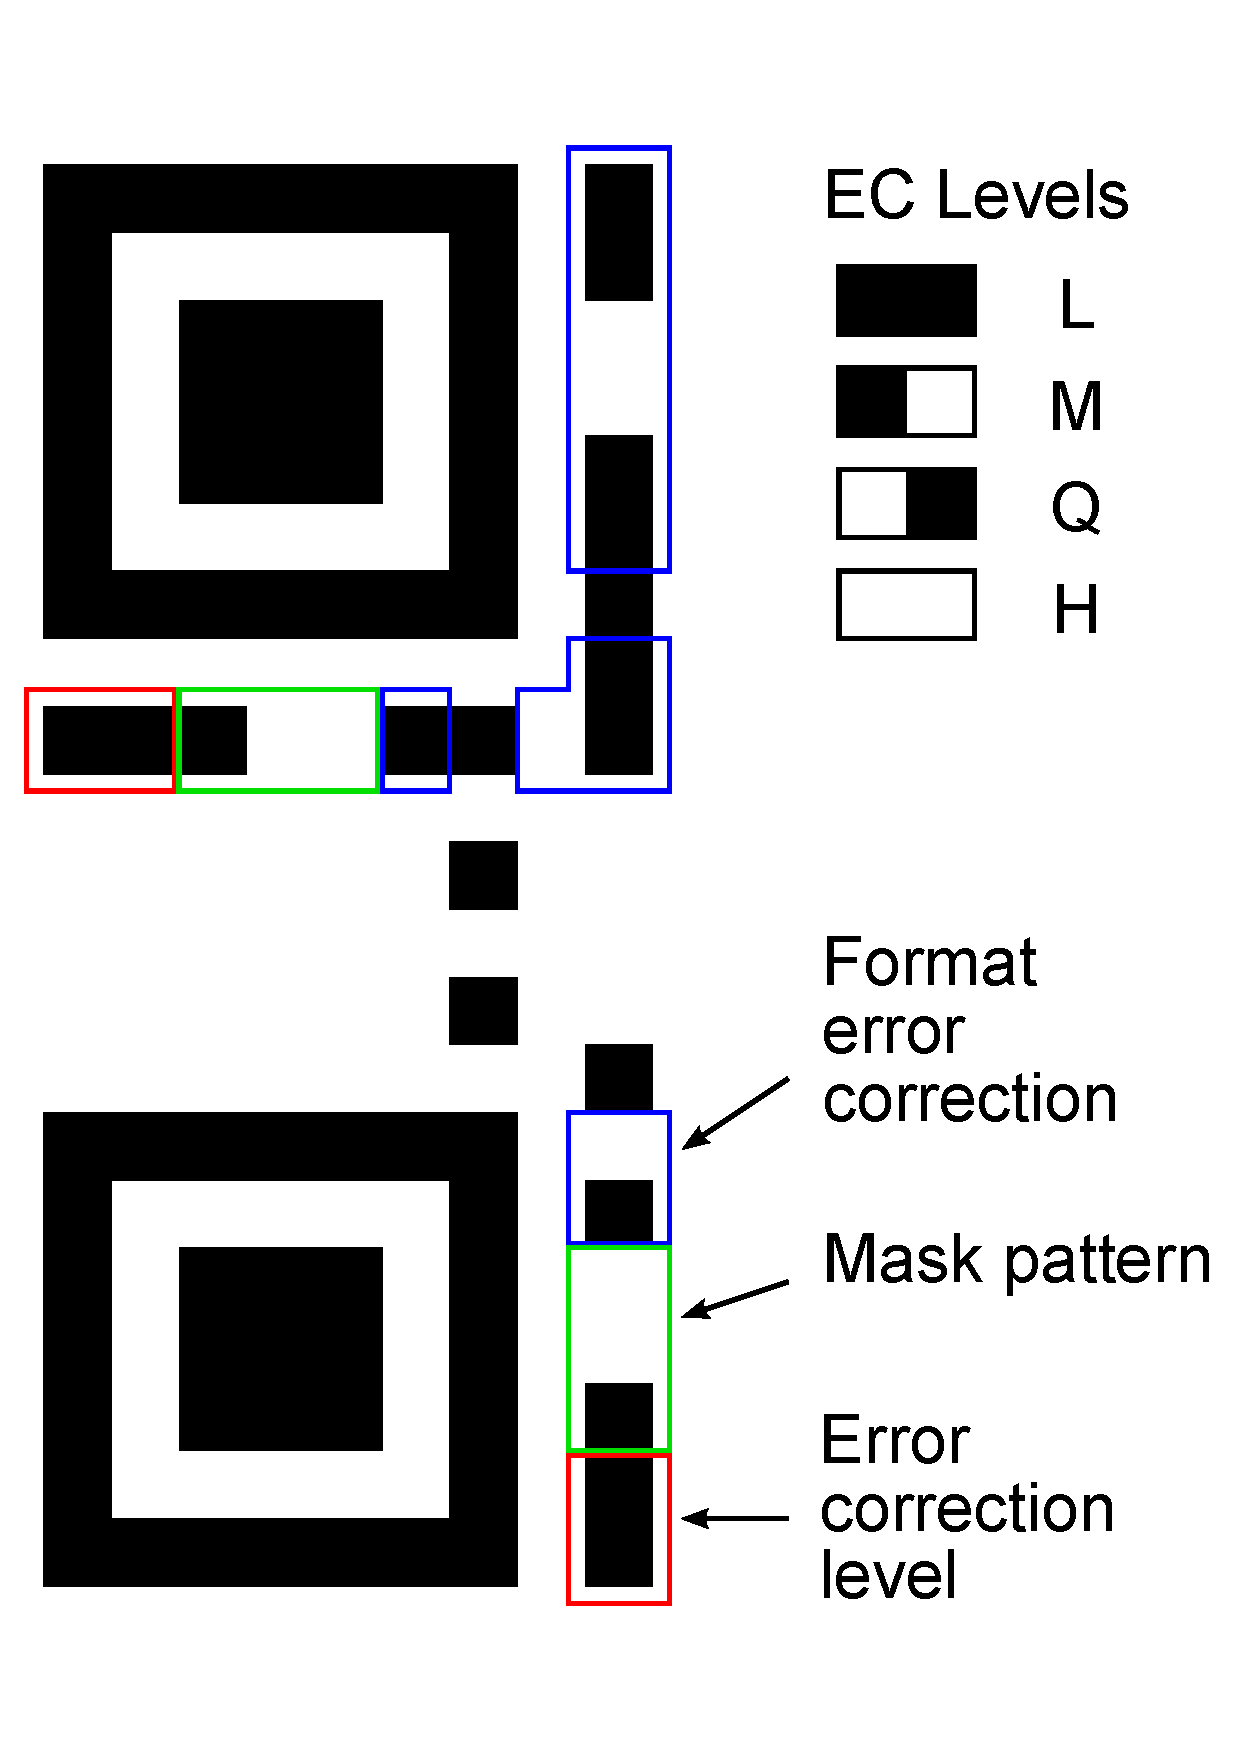
\includegraphics[height=0.4\textwidth]{figures/QR_Format_Information.pdf}
	\caption[Metadaten eines QR-Codes (Stufe L)]{Metadaten eines QR-Codes (Stufe L) \cite{QRCode2024}}
	\label{fig:qrschema}
\end{figure}
Die Nutzdaten sind, wie in Abbildung \ref{fig:qrdata} auf Seite \pageref{fig:qrdata} zu sehen, als Symbole mit je acht Modulen codiert.
Es können insgesamt 26 Symbole im QR-Code platziert werden.
Bei dem eingesetzten Reed-Solomon-Code $RS(255,248)$ gekürzt auf $RS(26,19)$ sind 19 Symbole für die Nutzdaten und sieben Symbole \textit{E1} bis \textit{E7} für die Fehlertoleranz.
Da zur Überprüfung nochmals zwei Symbole der Nachricht als Metadaten gebraucht werden, bleiben nur 17 der 19 Symbole für die eigentliche Nachricht \cite{pillazoHowDecodeQR2013}.
Damit können bis zu 2 Symbole also 16 Module korrigiert werden \cite{QRCode2024}.
\begin{figure}[ht]
	\centering
	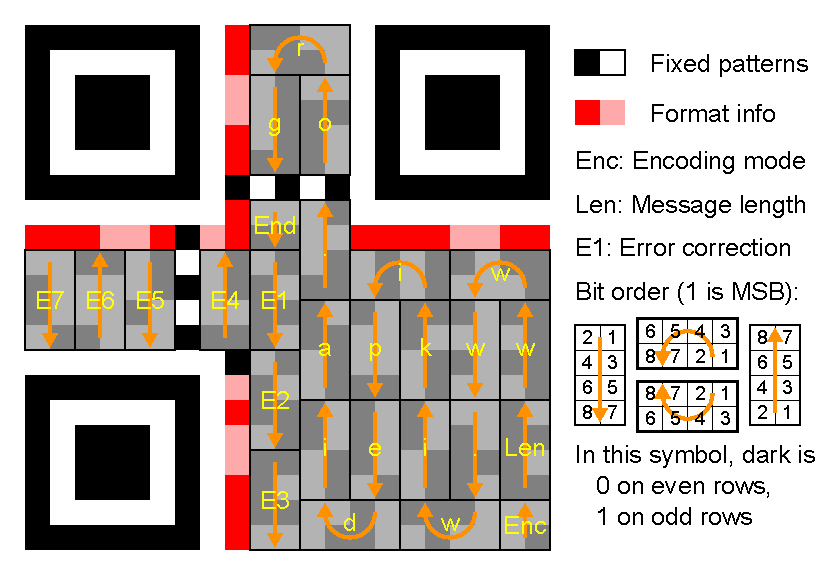
\includegraphics[height=0.4\textwidth]{figures/QR_Character_Placement.pdf}
	\caption[Datensymbole in einem QR-Code (Stufe L)]{Datensymbole in einem QR-Code (Stufe L) \cite{QRCode2024}}
	\label{fig:qrdata}
\end{figure}

Diese Fehlerkorrekturmechanismen verleihen QR-Codes Robustheit gegenüber physischen Beschädigungen wie Rissen, Kratzern oder Verunreinigungen. Die Fähigkeit, selbst unter solch herausfordernden Bedingungen die gespeicherten Daten korrekt wiederherzustellen, hat zur weitverbreiteten Nutzung von QR-Codes in verschiedenen Bereichen geführt, darunter Einzelhandel, Logistik und Zugangskontrollen \cite{QRCode2024}.